
\subsection{双亲委托模型(Parent Delegation Model)}

双亲委托模型翻译成“父委托模型”或“父委派模型”更加妥当。
如果一个类加载器收到了类加载的请求,它首先不会自己去尝试加载这个类,而是把请求委托给父加载器去完成,依次向上,因此,所有的类加载请求最终都应该被传递到顶层的启动类加载器中,只有当父加载器在它的搜索范围中没有找到所需的类时,即无法完成该加载,子加载器才会尝试自己去加载该类。
Java中ClassLoader的加载采用了双亲委托机制,采用双亲委托机制加载类的时候采用如下的几个步骤:

1.当前ClassLoader首先从自己已经加载的类中查询是否此类已经加载,如果已经加载则直接返回原来已经加载的类。每个类加载器都有自己的加载缓存,当一个类被加载了以后就会放入缓存,等下次加载的时候就可以直接返回了。

2.当前ClassLoader的缓存中没有找到被加载的类的时候,委托父类加载器去加载,父类加载器采用同样的策略,首先查看自己的缓存,然后委托父类的父类去加载,一直到BootStrap ClassLoader.

\begin{figure}[htbp]
	\centering
	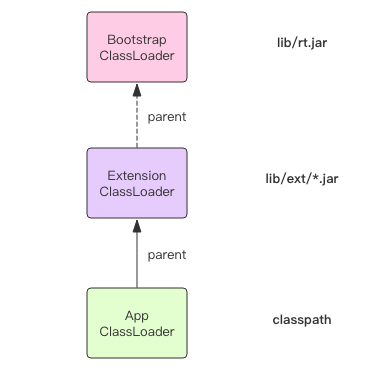
\includegraphics[scale=0.4]{classloader.png}
	\caption{Classloader}
	\label{fig:classloader}
\end{figure}

3.当所有的父类加载器都没有加载的时候,再由当前的类加载器加载,并将其放入它自己的缓存中,以便下次有加载请求的时候直接返回。

说到这里大家可能会想,Java为什么要采用这样的委托机制?理解这个问题,我们引入另外一个关于Classloader的概念“命名空间”, 它是指要确定某一个类,需要类的全限定名以及加载此类的ClassLoader来共同确定。也就是说即使两个类的全限定名是相同的,但是因为不同的ClassLoader加载了此类,那么在JVM中它是不同的类。明白了命名空间以后,我们再来看看委托模型。采用了委托模型以后加大了不同的 ClassLoader的交互能力,比如上面说的,我们JDK本生提供的类库,比如HashMap,LinkedList等等,这些类由BootStrap 类加载器加载了以后,无论你程序中有多少个类加载器,那么这些类其实都是可以共享的,这样就避免了不同的类加载器加载了同样名字的不同类以后造成混乱。

\paragraph{破坏父委托模型}

继承ClassLoader覆盖loadClass方法。原顺序第一是findLoadedClass,第二步委托parent加载器加载(这里注意bootstrap加载器的parent为null)。自行加载打破委派机制要做的就是打乱2和3的顺序,通过类名筛选自己要加载的类,其他的委托给parent加载器。使用线程上下文类加载器(Thread Context ClassLoader),在JVM中会把当前线程的类加载器加载不到的类交给线程上下文类加载器来加载,直接使用Thread.currentThread().getContextClassLoader()来获得,默认返回的就是应用程序类加载器,也可以通过java.lang.Thread类的setContextClassLoader()方法进行设置。而线程上下文类加载器破坏了双亲委派模型,也就是父类加载器请求子类加载器去完成类加载的动作,但为了实现功能,这也是一种巧妙的实现方式。
